\begin{figure*}[ht]
  \hspace*{-0.5cm}
  \begin{subfigure}{1.1\textwidth}
    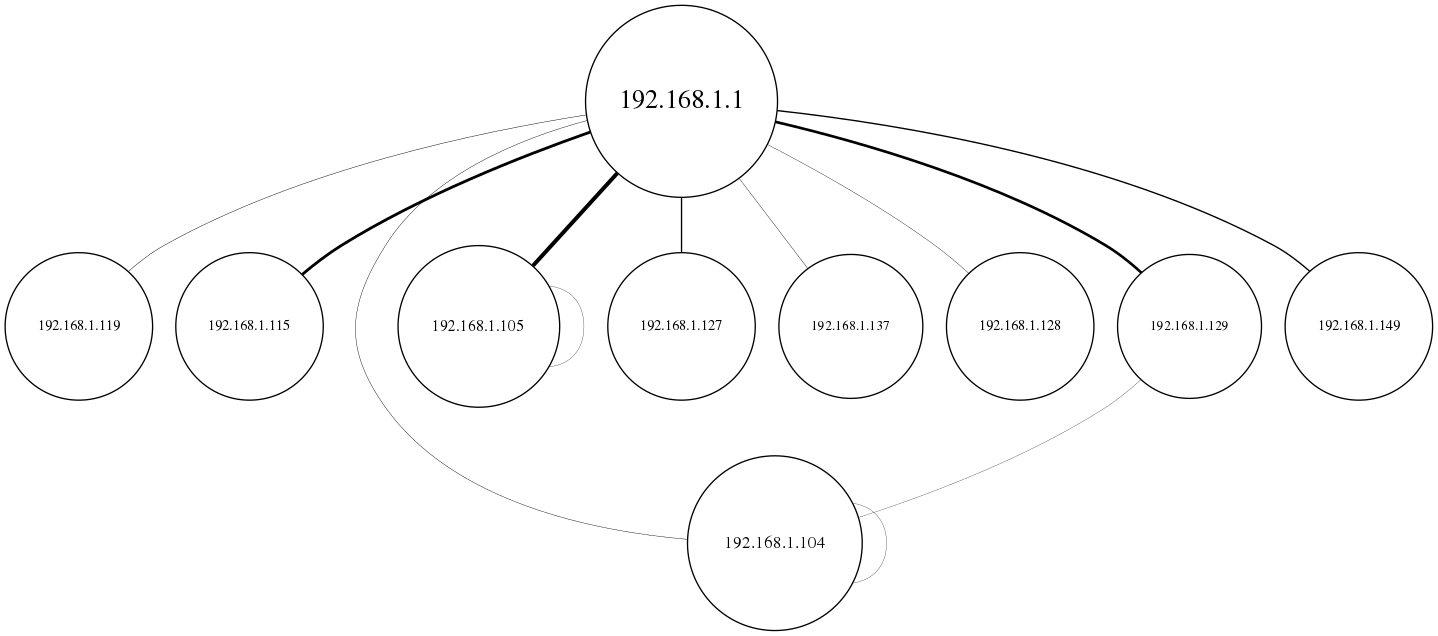
\includegraphics[width=\textwidth]{imagenes/hogarenia/grafo.png}
  \end{subfigure}
	\label{fig:exp2_hogar_grafo}
	\caption{Grafo con los nodos de la red de la segunda captura. El diámetro del nodo implica mayor participación en el envío de paquetes.}
\end{figure*}

\section{Segunda Captura: Red local chica}

\par Para una segunda experimentación, tomamos una captura de una red casera por medio de la herramienta sniffer antes mencionada. Se capturaron mensajes durante 2 horas y al ser una red pequeña, a diferencia del primer experimento, vamos a analizar tanto la fuente de información S como la S1.

\subsection{Resultados y análisis}

\par En el gráfico de la figura \ref{fig:exp2_hogar_hosts_infovsentro} podemos observar la información de cada símbolo (host) en la fuente S1. Se puede ver claramente que hay un solo host que se encuentra a la izquierda de la linea punteada roja, que representa la entropía de la red. Este host con IP \textbf{198.168.1.1} va a ser para nosotros un nodo distinguido, ya que participa fuértemente en los mensajes ARP que se envían en la red y por esto, tiene un valor de información pequeño.

\begin{figure}[h]
  \begin{subfigure}{.5\textwidth}
    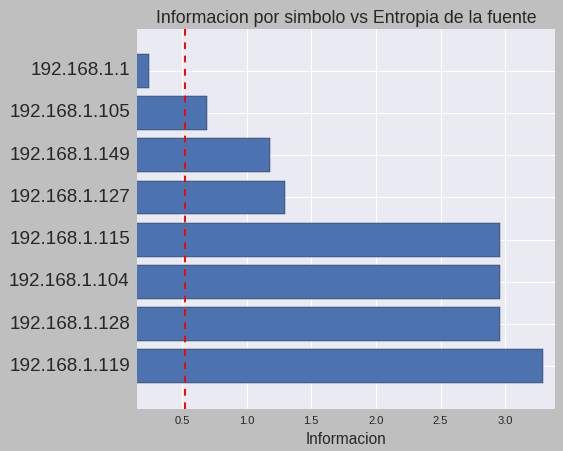
\includegraphics[width=\textwidth]{imagenes/hogarenia/hosts_informaciones_vs_entropia.png}
  \end{subfigure}
  \label{fig:exp2_hogar_hosts_infovsentro}
  \caption{Información de cada símbolo (host) comparada con el valor de la entropía de la fuente de información (red local).}
\end{figure}

\par Con respecto a la fuente de información S, tenemos el gráfico de la figura \ref{fig:exp2_hogar_brvsun_infovsentro}. En este gráfico observamos la información del símbolo \textit{Unicast} y el símbolo \textit{Broadcast}. Podemos notar que el símbolo \textit{Unicast} supera ampliamente al símbolo \textit{Broadcast}. Esto significa que se identificaron una cantidad elevada de mensajes del tipo \textit{Broadcast} en la red.

\begin{figure}[h]
  \begin{subfigure}{.5\textwidth}
    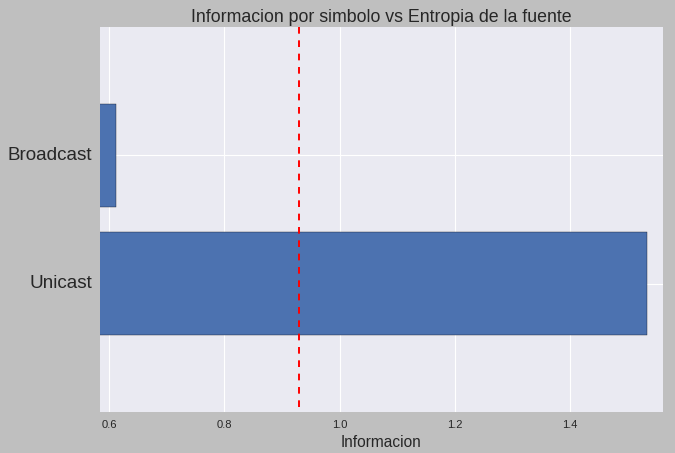
\includegraphics[width=\textwidth]{imagenes/hogarenia/brvsun_informaciones_vs_entropia.png}
  \end{subfigure}
  \label{fig:exp2_hogar_brvsun_infovsentro}
  \caption{Información de cada símbolo (Broadcas / Unicast) comparada con el valor de la entropía de la fuente de información (red local).}
\end{figure}

\par El grafo de la figura \ref{fig:exp2_hogar_grafo} es una representación de la red de acuerdo a los hosts identificados y las relaciones entre ellos (dadas por mensajes ARP que consultan direcciones entre ellos). El tamaño de los nodos, al igual que en la primer captura, está relacionado con la \textit{participación} que tienen en la red. Aquí también podemos notar que el host con IP \textbf{192.168.1.1} es el que mas participa de los mensajes ARP. También podemos notar que todos los otros hosts se encuentran unidos a él (preguntaron por su dirección o la inversa). De el mismo grafo, podemos ver también que los hosts \textbf{192.168.1.104} y \textbf{192.168.1.129} se encuentran conectados, mientras que todo el resto solo se conectan con el host \textbf{192.168.1.1}. Luego de corroborar los datos, notamos que hay un mensaje ARP que emitió el host \textbf{192.168.1.104} preguntando por la dirección del host \textbf{192.168.1.129}.

\subsection{Conclusiones}

\par Como observamos en el grafo y corroboramos con la información del símbolo en la fuente de información S, el host \textbf{192.168.1.1} se encuentra conectado con todos los otros hosts, por lo que creemos que es un router o access point con el cual el resto de los hosts se comunican. El resto de los hosts, nos resultan similares y no creemos que sean hosts destacados o distinguidos.
